\documentclass[twoside]{article}

% Packages required by doxygen
\usepackage{calc}
\usepackage{doxygen}
\usepackage{graphicx}
\usepackage[utf8]{inputenc}
\usepackage{makeidx}
\usepackage{multicol}
\usepackage{multirow}
\usepackage{textcomp}
\usepackage[table]{xcolor}

% Font selection
\usepackage[T1]{fontenc}
\usepackage{mathptmx}
\usepackage[scaled=.90]{helvet}
\usepackage{courier}
\usepackage{amssymb}
\usepackage{sectsty}
\renewcommand{\familydefault}{\sfdefault}
\allsectionsfont{%
  \fontseries{bc}\selectfont%
  \color{darkgray}%
}
\renewcommand{\DoxyLabelFont}{%
  \fontseries{bc}\selectfont%
  \color{darkgray}%
}

% Page & text layout
\usepackage{geometry}
\geometry{%
  a4paper,%
  top=2.5cm,%
  bottom=2.5cm,%
  left=2.5cm,%
  right=2.5cm%
}
\tolerance=750
\hfuzz=15pt
\hbadness=750
\setlength{\emergencystretch}{15pt}
\setlength{\parindent}{0cm}
\setlength{\parskip}{0.2cm}
\makeatletter
\renewcommand{\paragraph}{%
  \@startsection{paragraph}{4}{0ex}{-1.0ex}{1.0ex}{%
    \normalfont\normalsize\bfseries\SS@parafont%
  }%
}
\renewcommand{\subparagraph}{%
  \@startsection{subparagraph}{5}{0ex}{-1.0ex}{1.0ex}{%
    \normalfont\normalsize\bfseries\SS@subparafont%
  }%
}
\makeatother

% Headers & footers
\usepackage{fancyhdr}
\pagestyle{fancyplain}
\fancyhead[LE]{\fancyplain{}{\bfseries\thepage}}
\fancyhead[CE]{\fancyplain{}{}}
\fancyhead[RE]{\fancyplain{}{\bfseries\leftmark}}
\fancyhead[LO]{\fancyplain{}{\bfseries\rightmark}}
\fancyhead[CO]{\fancyplain{}{}}
\fancyhead[RO]{\fancyplain{}{\bfseries\thepage}}
\fancyfoot[LE]{\fancyplain{}{}}
\fancyfoot[CE]{\fancyplain{}{}}
\fancyfoot[RE]{\fancyplain{}{\bfseries\scriptsize Generated on Wed Sep 14 2016 20\-:53\-:54 for P\-A01 by Doxygen }}
\fancyfoot[LO]{\fancyplain{}{\bfseries\scriptsize Generated on Wed Sep 14 2016 20\-:53\-:54 for P\-A01 by Doxygen }}
\fancyfoot[CO]{\fancyplain{}{}}
\fancyfoot[RO]{\fancyplain{}{}}
\renewcommand{\footrulewidth}{0.4pt}
\renewcommand{\sectionmark}[1]{%
  \markright{\thesection\ #1}%
}

% Indices & bibliography
\usepackage{natbib}
\usepackage[titles]{tocloft}
\setcounter{tocdepth}{3}
\setcounter{secnumdepth}{5}
\makeindex

% Hyperlinks (required, but should be loaded last)
\usepackage{ifpdf}
\ifpdf
  \usepackage[pdftex,pagebackref=true]{hyperref}
\else
  \usepackage[ps2pdf,pagebackref=true]{hyperref}
\fi
\hypersetup{%
  colorlinks=true,%
  linkcolor=blue,%
  citecolor=blue,%
  unicode%
}

% Custom commands
\newcommand{\clearemptydoublepage}{%
  \newpage{\pagestyle{empty}\cleardoublepage}%
}


%===== C O N T E N T S =====

\begin{document}

% Titlepage & ToC
\hypersetup{pageanchor=false}
\pagenumbering{roman}
\begin{titlepage}
\vspace*{7cm}
\begin{center}%
{\Large P\-A01 }\\
\vspace*{1cm}
{\large Generated by Doxygen 1.8.6}\\
\vspace*{0.5cm}
{\small Wed Sep 14 2016 20:53:54}\\
\end{center}
\end{titlepage}
\tableofcontents
\pagenumbering{arabic}
\hypersetup{pageanchor=true}

%--- Begin generated contents ---
\section{Hierarchical Index}
\subsection{Class Hierarchy}
This inheritance list is sorted roughly, but not completely, alphabetically\-:\begin{DoxyCompactList}
\item \contentsline{section}{List\-Interface$<$ Item\-Type $>$}{\pageref{class_list_interface}}{}
\begin{DoxyCompactList}
\item \contentsline{section}{Linked\-List$<$ Item\-Type $>$}{\pageref{class_linked_list}}{}
\end{DoxyCompactList}
\item logic\-\_\-error\begin{DoxyCompactList}
\item \contentsline{section}{Precond\-Violated\-Except}{\pageref{class_precond_violated_except}}{}
\end{DoxyCompactList}
\item \contentsline{section}{Node$<$ Item\-Type $>$}{\pageref{class_node}}{}
\end{DoxyCompactList}

\section{Class Index}
\subsection{Class List}
Here are the classes, structs, unions and interfaces with brief descriptions\-:\begin{DoxyCompactList}
\item\contentsline{section}{\hyperlink{class_linked_list}{Linked\-List$<$ Item\-Type $>$} }{\pageref{class_linked_list}}{}
\item\contentsline{section}{\hyperlink{class_list_interface}{List\-Interface$<$ Item\-Type $>$} }{\pageref{class_list_interface}}{}
\item\contentsline{section}{\hyperlink{class_node}{Node$<$ Item\-Type $>$} }{\pageref{class_node}}{}
\item\contentsline{section}{\hyperlink{class_precond_violated_except}{Precond\-Violated\-Except} }{\pageref{class_precond_violated_except}}{}
\end{DoxyCompactList}

\section{File Index}
\subsection{File List}
Here is a list of all documented files with brief descriptions\+:\begin{DoxyCompactList}
\item\contentsline{section}{\hyperlink{_array_queue_8cpp}{Array\+Queue.\+cpp} }{\pageref{_array_queue_8cpp}}{}
\item\contentsline{section}{\hyperlink{_array_queue_8h}{Array\+Queue.\+h} }{\pageref{_array_queue_8h}}{}
\item\contentsline{section}{{\bfseries Event.\+h} }{\pageref{_event_8h}}{}
\item\contentsline{section}{\hyperlink{_linked_list_8cpp}{Linked\+List.\+cpp} }{\pageref{_linked_list_8cpp}}{}
\item\contentsline{section}{\hyperlink{_linked_list_8h}{Linked\+List.\+h} \\*Header file for a linked list }{\pageref{_linked_list_8h}}{}
\item\contentsline{section}{\hyperlink{_linked_queue_8h}{Linked\+Queue.\+h} }{\pageref{_linked_queue_8h}}{}
\item\contentsline{section}{\hyperlink{_list_interface_8h}{List\+Interface.\+h} \\*Interface file for the List A\+DT }{\pageref{_list_interface_8h}}{}
\item\contentsline{section}{\hyperlink{_node_8cpp}{Node.\+cpp} }{\pageref{_node_8cpp}}{}
\item\contentsline{section}{\hyperlink{_node_8h}{Node.\+h} }{\pageref{_node_8h}}{}
\item\contentsline{section}{\hyperlink{_precond_violated_except_8cpp}{Precond\+Violated\+Except.\+cpp} }{\pageref{_precond_violated_except_8cpp}}{}
\item\contentsline{section}{\hyperlink{_precond_violated_except_8h}{Precond\+Violated\+Except.\+h} }{\pageref{_precond_violated_except_8h}}{}
\item\contentsline{section}{\hyperlink{_priority_queue_interface_8h}{Priority\+Queue\+Interface.\+h} }{\pageref{_priority_queue_interface_8h}}{}
\item\contentsline{section}{\hyperlink{_queue_interface_8h}{Queue\+Interface.\+h} }{\pageref{_queue_interface_8h}}{}
\item\contentsline{section}{\hyperlink{_s_l___priority_queue_8h}{S\+L\+\_\+\+Priority\+Queue.\+h} }{\pageref{_s_l___priority_queue_8h}}{}
\item\contentsline{section}{\hyperlink{_sorted_list_interface_8h}{Sorted\+List\+Interface.\+h} }{\pageref{_sorted_list_interface_8h}}{}
\item\contentsline{section}{\hyperlink{_sorted_list_is_a_8h}{Sorted\+List\+Is\+A.\+h} }{\pageref{_sorted_list_is_a_8h}}{}
\end{DoxyCompactList}

\section{Class Documentation}
\hypertarget{class_linked_list}{}\subsection{Linked\+List$<$ Item\+Type $>$ Class Template Reference}
\label{class_linked_list}\index{Linked\+List$<$ Item\+Type $>$@{Linked\+List$<$ Item\+Type $>$}}
Inheritance diagram for Linked\+List$<$ Item\+Type $>$\+:\begin{figure}[H]
\begin{center}
\leavevmode
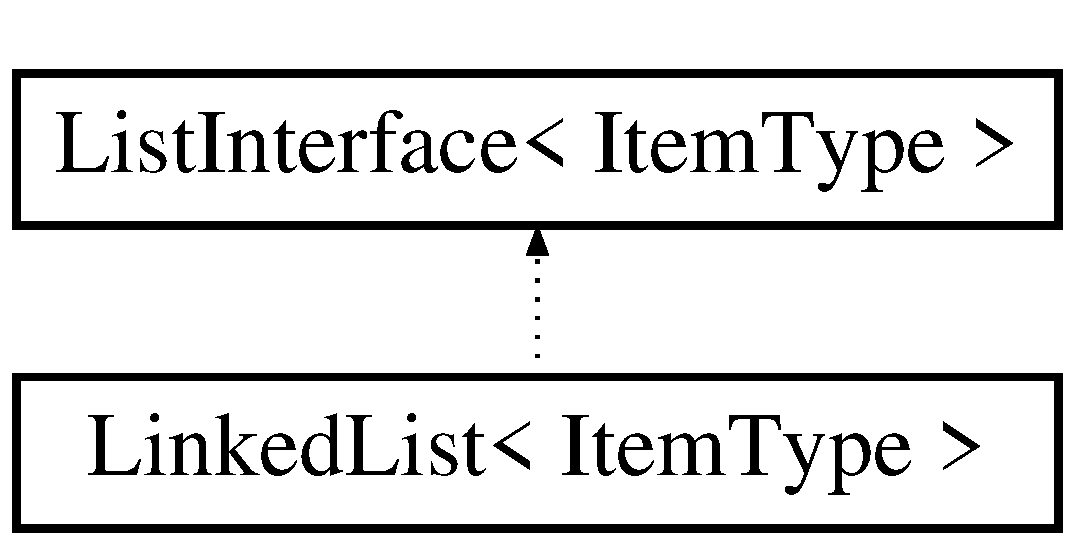
\includegraphics[height=3.000000cm]{class_linked_list}
\end{center}
\end{figure}
\subsubsection*{Public Member Functions}
\begin{DoxyCompactItemize}
\item 
\hyperlink{class_linked_list_adf8d8164e06b6d358a36df7e53e814ee}{Linked\+List} ()
\item 
\hyperlink{class_linked_list_a6f1443c6120352f1f5b6bd3c0d95e41e}{Linked\+List} (const \hyperlink{class_linked_list}{Linked\+List}$<$ Item\+Type $>$ \&a\+List)
\item 
virtual \hyperlink{class_linked_list_a66aee17d756fe0e002375897383c180b}{$\sim$\+Linked\+List} ()
\item 
bool \hyperlink{class_linked_list_adb17aed0ceacbbe1f247d235f491f0d5}{is\+Empty} () const 
\item 
int \hyperlink{class_linked_list_adae55d6b79235c816cb9e05027fd2e7a}{get\+Length} () const 
\item 
bool \hyperlink{class_linked_list_ae8a19375505e87e2e4fc0e9b5afe4d4d}{insert} (int new\+Position, const Item\+Type \&new\+Entry)
\item 
bool \hyperlink{class_linked_list_a16a02716b5b2efb6fb1e3d18721b53e4}{remove} (int position)
\item 
void \hyperlink{class_linked_list_a7d1d9cf83eef67b6c4d700a3cc5970e1}{clear} ()
\item 
Item\+Type \hyperlink{class_linked_list_a79f005e696c19f6ccf90d9d535afa999}{get\+Entry} (int position) const   throw (\+Precond\+Violated\+Except)
\item 
void \hyperlink{class_linked_list_a3035f880c50e7d8f68e67c093d4607ca}{replace} (int position, const Item\+Type \&new\+Entry)  throw (\+Precond\+Violated\+Except)
\end{DoxyCompactItemize}


\subsubsection{Constructor \& Destructor Documentation}
\index{Linked\+List@{Linked\+List}!Linked\+List@{Linked\+List}}
\index{Linked\+List@{Linked\+List}!Linked\+List@{Linked\+List}}
\paragraph[{\texorpdfstring{Linked\+List()}{LinkedList()}}]{\setlength{\rightskip}{0pt plus 5cm}template$<$class Item\+Type $>$ {\bf Linked\+List}$<$ Item\+Type $>$\+::{\bf Linked\+List} (
\begin{DoxyParamCaption}
{}
\end{DoxyParamCaption}
)}\hypertarget{class_linked_list_adf8d8164e06b6d358a36df7e53e814ee}{}\label{class_linked_list_adf8d8164e06b6d358a36df7e53e814ee}
default constructor \index{Linked\+List@{Linked\+List}!Linked\+List@{Linked\+List}}
\index{Linked\+List@{Linked\+List}!Linked\+List@{Linked\+List}}
\paragraph[{\texorpdfstring{Linked\+List(const Linked\+List$<$ Item\+Type $>$ \&a\+List)}{LinkedList(const LinkedList< ItemType > &aList)}}]{\setlength{\rightskip}{0pt plus 5cm}template$<$class Item\+Type $>$ {\bf Linked\+List}$<$ Item\+Type $>$\+::{\bf Linked\+List} (
\begin{DoxyParamCaption}
\item[{const {\bf Linked\+List}$<$ Item\+Type $>$ \&}]{a\+List}
\end{DoxyParamCaption}
)}\hypertarget{class_linked_list_a6f1443c6120352f1f5b6bd3c0d95e41e}{}\label{class_linked_list_a6f1443c6120352f1f5b6bd3c0d95e41e}
copy constructor \index{Linked\+List@{Linked\+List}!````~Linked\+List@{$\sim$\+Linked\+List}}
\index{````~Linked\+List@{$\sim$\+Linked\+List}!Linked\+List@{Linked\+List}}
\paragraph[{\texorpdfstring{$\sim$\+Linked\+List()}{~LinkedList()}}]{\setlength{\rightskip}{0pt plus 5cm}template$<$class Item\+Type $>$ {\bf Linked\+List}$<$ Item\+Type $>$\+::$\sim${\bf Linked\+List} (
\begin{DoxyParamCaption}
{}
\end{DoxyParamCaption}
)\hspace{0.3cm}{\ttfamily [virtual]}}\hypertarget{class_linked_list_a66aee17d756fe0e002375897383c180b}{}\label{class_linked_list_a66aee17d756fe0e002375897383c180b}
destructor 

\subsubsection{Member Function Documentation}
\index{Linked\+List@{Linked\+List}!clear@{clear}}
\index{clear@{clear}!Linked\+List@{Linked\+List}}
\paragraph[{\texorpdfstring{clear()}{clear()}}]{\setlength{\rightskip}{0pt plus 5cm}template$<$class Item\+Type $>$ void {\bf Linked\+List}$<$ Item\+Type $>$\+::clear (
\begin{DoxyParamCaption}
{}
\end{DoxyParamCaption}
)\hspace{0.3cm}{\ttfamily [virtual]}}\hypertarget{class_linked_list_a7d1d9cf83eef67b6c4d700a3cc5970e1}{}\label{class_linked_list_a7d1d9cf83eef67b6c4d700a3cc5970e1}
removes all items from the list. \begin{DoxyPrecond}{Precondition}
None. 
\end{DoxyPrecond}
\begin{DoxyPostcond}{Postcondition}
List contains no entries. 
\end{DoxyPostcond}


Implements \hyperlink{class_list_interface_adfda414908b645bdf19bcab8269168b7}{List\+Interface$<$ Item\+Type $>$}.

\index{Linked\+List@{Linked\+List}!get\+Entry@{get\+Entry}}
\index{get\+Entry@{get\+Entry}!Linked\+List@{Linked\+List}}
\paragraph[{\texorpdfstring{get\+Entry(int position) const }{getEntry(int position) const }}]{\setlength{\rightskip}{0pt plus 5cm}template$<$class Item\+Type $>$ Item\+Type {\bf Linked\+List}$<$ Item\+Type $>$\+::get\+Entry (
\begin{DoxyParamCaption}
\item[{int}]{position}
\end{DoxyParamCaption}
) const throw  {\bf Precond\+Violated\+Except}) \hspace{0.3cm}{\ttfamily [virtual]}}\hypertarget{class_linked_list_a79f005e696c19f6ccf90d9d535afa999}{}\label{class_linked_list_a79f005e696c19f6ccf90d9d535afa999}
Gets the entry at the given position in this list. \begin{DoxyPrecond}{Precondition}
1 $<$= position $<$= \hyperlink{class_linked_list_adae55d6b79235c816cb9e05027fd2e7a}{get\+Length()}. 
\end{DoxyPrecond}
\begin{DoxyPostcond}{Postcondition}
The desired entry has been returned. 
\end{DoxyPostcond}

\begin{DoxyParams}{Parameters}
{\em position} & The list position of the desired entry. \\
\hline
\end{DoxyParams}
\begin{DoxyReturn}{Returns}
The entry at the given position. 
\end{DoxyReturn}

\begin{DoxyExceptions}{Exceptions}
{\em \hyperlink{class_precond_violated_except}{Precond\+Violated\+Except}} & if position $<$ 1 or position $>$ \hyperlink{class_linked_list_adae55d6b79235c816cb9e05027fd2e7a}{get\+Length()}. \\
\hline
\end{DoxyExceptions}


Implements \hyperlink{class_list_interface_a86987f69e5056d287212ede41db1956a}{List\+Interface$<$ Item\+Type $>$}.

\index{Linked\+List@{Linked\+List}!get\+Length@{get\+Length}}
\index{get\+Length@{get\+Length}!Linked\+List@{Linked\+List}}
\paragraph[{\texorpdfstring{get\+Length() const }{getLength() const }}]{\setlength{\rightskip}{0pt plus 5cm}template$<$class Item\+Type $>$ int {\bf Linked\+List}$<$ Item\+Type $>$\+::get\+Length (
\begin{DoxyParamCaption}
{}
\end{DoxyParamCaption}
) const\hspace{0.3cm}{\ttfamily [virtual]}}\hypertarget{class_linked_list_adae55d6b79235c816cb9e05027fd2e7a}{}\label{class_linked_list_adae55d6b79235c816cb9e05027fd2e7a}
checks how many items are in the list \begin{DoxyReturn}{Returns}
the integer value of how many items are contained in the list. 
\end{DoxyReturn}


Implements \hyperlink{class_list_interface_afc85695d4137f1e29ff02e179c9f3221}{List\+Interface$<$ Item\+Type $>$}.

\index{Linked\+List@{Linked\+List}!insert@{insert}}
\index{insert@{insert}!Linked\+List@{Linked\+List}}
\paragraph[{\texorpdfstring{insert(int new\+Position, const Item\+Type \&new\+Entry)}{insert(int newPosition, const ItemType &newEntry)}}]{\setlength{\rightskip}{0pt plus 5cm}template$<$class Item\+Type $>$ bool {\bf Linked\+List}$<$ Item\+Type $>$\+::insert (
\begin{DoxyParamCaption}
\item[{int}]{new\+Position, }
\item[{const Item\+Type \&}]{new\+Entry}
\end{DoxyParamCaption}
)\hspace{0.3cm}{\ttfamily [virtual]}}\hypertarget{class_linked_list_ae8a19375505e87e2e4fc0e9b5afe4d4d}{}\label{class_linked_list_ae8a19375505e87e2e4fc0e9b5afe4d4d}
inserts an entry into the list at a given position \begin{DoxyPrecond}{Precondition}
None. 
\end{DoxyPrecond}
\begin{DoxyPostcond}{Postcondition}
if the position is valid and insertion is possible a new entry is entered into the list. 
\end{DoxyPostcond}

\begin{DoxyParams}{Parameters}
{\em new\+Position} & the position in the list at which to insert the new entry. \\
\hline
{\em new\+Entry} & the new item to be placed in the list. \\
\hline
\end{DoxyParams}
\begin{DoxyReturn}{Returns}
True if the item was successfully placed in the list. 
\end{DoxyReturn}


Implements \hyperlink{class_list_interface_a5b2f86954a86172699a3495982c38e77}{List\+Interface$<$ Item\+Type $>$}.



Reimplemented in \hyperlink{class_sorted_list_is_a_aa80ef5215183e3a17f2a2f2e76d4fca3}{Sorted\+List\+Is\+A$<$ Item\+Type $>$}.

\index{Linked\+List@{Linked\+List}!is\+Empty@{is\+Empty}}
\index{is\+Empty@{is\+Empty}!Linked\+List@{Linked\+List}}
\paragraph[{\texorpdfstring{is\+Empty() const }{isEmpty() const }}]{\setlength{\rightskip}{0pt plus 5cm}template$<$class Item\+Type $>$ bool {\bf Linked\+List}$<$ Item\+Type $>$\+::is\+Empty (
\begin{DoxyParamCaption}
{}
\end{DoxyParamCaption}
) const\hspace{0.3cm}{\ttfamily [virtual]}}\hypertarget{class_linked_list_adb17aed0ceacbbe1f247d235f491f0d5}{}\label{class_linked_list_adb17aed0ceacbbe1f247d235f491f0d5}
checks if the list contains any items \begin{DoxyReturn}{Returns}
returns true if the list is empty. 
\end{DoxyReturn}


Implements \hyperlink{class_list_interface_a924f91e7f81d7dcd3fda79bbcc671394}{List\+Interface$<$ Item\+Type $>$}.

\index{Linked\+List@{Linked\+List}!remove@{remove}}
\index{remove@{remove}!Linked\+List@{Linked\+List}}
\paragraph[{\texorpdfstring{remove(int position)}{remove(int position)}}]{\setlength{\rightskip}{0pt plus 5cm}template$<$class Item\+Type $>$ bool {\bf Linked\+List}$<$ Item\+Type $>$\+::remove (
\begin{DoxyParamCaption}
\item[{int}]{position}
\end{DoxyParamCaption}
)\hspace{0.3cm}{\ttfamily [virtual]}}\hypertarget{class_linked_list_a16a02716b5b2efb6fb1e3d18721b53e4}{}\label{class_linked_list_a16a02716b5b2efb6fb1e3d18721b53e4}
removes the entry at the specified position. \begin{DoxyPrecond}{Precondition}
None. 
\end{DoxyPrecond}
\begin{DoxyPostcond}{Postcondition}
if the position is valid the item is removed from the list and the list is renumbered. 
\end{DoxyPostcond}

\begin{DoxyParams}{Parameters}
{\em position} & the position in the list which contains the item to be removed. \\
\hline
\end{DoxyParams}
\begin{DoxyReturn}{Returns}
True if the item was removed succesfully otherwise returns false. 
\end{DoxyReturn}


Implements \hyperlink{class_list_interface_a5543002ec0d64bd2a63f3732f437af65}{List\+Interface$<$ Item\+Type $>$}.

\index{Linked\+List@{Linked\+List}!replace@{replace}}
\index{replace@{replace}!Linked\+List@{Linked\+List}}
\paragraph[{\texorpdfstring{replace(int position, const Item\+Type \&new\+Entry)}{replace(int position, const ItemType &newEntry)}}]{\setlength{\rightskip}{0pt plus 5cm}template$<$class Item\+Type $>$ void {\bf Linked\+List}$<$ Item\+Type $>$\+::replace (
\begin{DoxyParamCaption}
\item[{int}]{position, }
\item[{const Item\+Type \&}]{new\+Entry}
\end{DoxyParamCaption}
) throw  {\bf Precond\+Violated\+Except}) \hspace{0.3cm}{\ttfamily [virtual]}}\hypertarget{class_linked_list_a3035f880c50e7d8f68e67c093d4607ca}{}\label{class_linked_list_a3035f880c50e7d8f68e67c093d4607ca}
Replaces the entry at the given position in this list. \begin{DoxyPrecond}{Precondition}
1 $<$= position $<$= \hyperlink{class_linked_list_adae55d6b79235c816cb9e05027fd2e7a}{get\+Length()}. 
\end{DoxyPrecond}
\begin{DoxyPostcond}{Postcondition}
The entry at the given position is new\+Entry. 
\end{DoxyPostcond}

\begin{DoxyParams}{Parameters}
{\em position} & The list position of the entry to replace. \\
\hline
{\em new\+Entry} & The replacement entry. \\
\hline
\end{DoxyParams}

\begin{DoxyExceptions}{Exceptions}
{\em \hyperlink{class_precond_violated_except}{Precond\+Violated\+Except}} & if position $<$ 1 or position $>$ \hyperlink{class_linked_list_adae55d6b79235c816cb9e05027fd2e7a}{get\+Length()}. \\
\hline
\end{DoxyExceptions}


Implements \hyperlink{class_list_interface_aae877a56b7b9f5f526c37a00e234fad1}{List\+Interface$<$ Item\+Type $>$}.



Reimplemented in \hyperlink{class_sorted_list_is_a_ae85cca0f8a4a306d6d28cc5993e5895c}{Sorted\+List\+Is\+A$<$ Item\+Type $>$}.



The documentation for this class was generated from the following files\+:\begin{DoxyCompactItemize}
\item 
\hyperlink{_linked_list_8h}{Linked\+List.\+h}\item 
\hyperlink{_linked_list_8cpp}{Linked\+List.\+cpp}\end{DoxyCompactItemize}

\hypertarget{class_list_interface}{}\subsection{List\+Interface$<$ Item\+Type $>$ Class Template Reference}
\label{class_list_interface}\index{List\+Interface$<$ Item\+Type $>$@{List\+Interface$<$ Item\+Type $>$}}
Inheritance diagram for List\+Interface$<$ Item\+Type $>$\+:\begin{figure}[H]
\begin{center}
\leavevmode
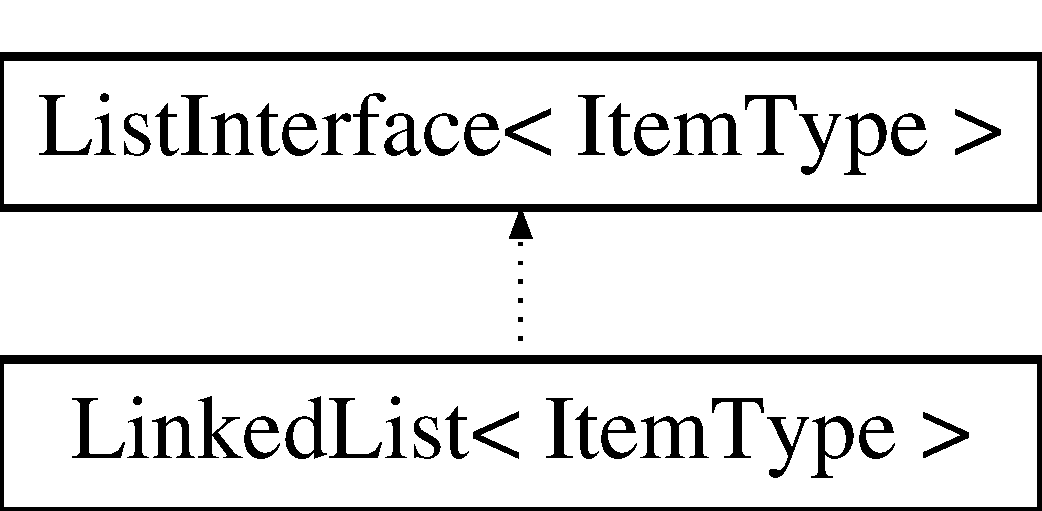
\includegraphics[height=3.000000cm]{class_list_interface}
\end{center}
\end{figure}
\subsubsection*{Public Member Functions}
\begin{DoxyCompactItemize}
\item 
virtual bool \hyperlink{class_list_interface_a924f91e7f81d7dcd3fda79bbcc671394}{is\+Empty} () const =0
\item 
virtual int \hyperlink{class_list_interface_afc85695d4137f1e29ff02e179c9f3221}{get\+Length} () const =0
\item 
virtual bool \hyperlink{class_list_interface_a5b2f86954a86172699a3495982c38e77}{insert} (int new\+Position, const Item\+Type \&new\+Entry)=0
\item 
virtual bool \hyperlink{class_list_interface_a5543002ec0d64bd2a63f3732f437af65}{remove} (int position)=0
\item 
virtual void \hyperlink{class_list_interface_adfda414908b645bdf19bcab8269168b7}{clear} ()=0
\item 
virtual Item\+Type \hyperlink{class_list_interface_a86987f69e5056d287212ede41db1956a}{get\+Entry} (int position) const =0
\item 
virtual void \hyperlink{class_list_interface_aae877a56b7b9f5f526c37a00e234fad1}{replace} (int position, const Item\+Type \&new\+Entry)=0
\end{DoxyCompactItemize}


\subsubsection{Member Function Documentation}
\index{List\+Interface@{List\+Interface}!clear@{clear}}
\index{clear@{clear}!List\+Interface@{List\+Interface}}
\paragraph[{\texorpdfstring{clear()=0}{clear()=0}}]{\setlength{\rightskip}{0pt plus 5cm}template$<$class Item\+Type $>$ virtual void {\bf List\+Interface}$<$ Item\+Type $>$\+::clear (
\begin{DoxyParamCaption}
{}
\end{DoxyParamCaption}
)\hspace{0.3cm}{\ttfamily [pure virtual]}}\hypertarget{class_list_interface_adfda414908b645bdf19bcab8269168b7}{}\label{class_list_interface_adfda414908b645bdf19bcab8269168b7}
Removes all entries from this list. \begin{DoxyPostcond}{Postcondition}
List contains no entries and the count of items is 0. 
\end{DoxyPostcond}


Implemented in \hyperlink{class_linked_list_a7d1d9cf83eef67b6c4d700a3cc5970e1}{Linked\+List$<$ Item\+Type $>$}.

\index{List\+Interface@{List\+Interface}!get\+Entry@{get\+Entry}}
\index{get\+Entry@{get\+Entry}!List\+Interface@{List\+Interface}}
\paragraph[{\texorpdfstring{get\+Entry(int position) const =0}{getEntry(int position) const =0}}]{\setlength{\rightskip}{0pt plus 5cm}template$<$class Item\+Type $>$ virtual Item\+Type {\bf List\+Interface}$<$ Item\+Type $>$\+::get\+Entry (
\begin{DoxyParamCaption}
\item[{int}]{position}
\end{DoxyParamCaption}
) const\hspace{0.3cm}{\ttfamily [pure virtual]}}\hypertarget{class_list_interface_a86987f69e5056d287212ede41db1956a}{}\label{class_list_interface_a86987f69e5056d287212ede41db1956a}
Gets the entry at the given position in this list. \begin{DoxyPrecond}{Precondition}
1 $<$= position $<$= \hyperlink{class_list_interface_afc85695d4137f1e29ff02e179c9f3221}{get\+Length()}. 
\end{DoxyPrecond}
\begin{DoxyPostcond}{Postcondition}
The desired entry has been returned. 
\end{DoxyPostcond}

\begin{DoxyParams}{Parameters}
{\em position} & The list position of the desired entry. \\
\hline
\end{DoxyParams}
\begin{DoxyReturn}{Returns}
The entry at the given position. 
\end{DoxyReturn}


Implemented in \hyperlink{class_linked_list_a79f005e696c19f6ccf90d9d535afa999}{Linked\+List$<$ Item\+Type $>$}.

\index{List\+Interface@{List\+Interface}!get\+Length@{get\+Length}}
\index{get\+Length@{get\+Length}!List\+Interface@{List\+Interface}}
\paragraph[{\texorpdfstring{get\+Length() const =0}{getLength() const =0}}]{\setlength{\rightskip}{0pt plus 5cm}template$<$class Item\+Type $>$ virtual int {\bf List\+Interface}$<$ Item\+Type $>$\+::get\+Length (
\begin{DoxyParamCaption}
{}
\end{DoxyParamCaption}
) const\hspace{0.3cm}{\ttfamily [pure virtual]}}\hypertarget{class_list_interface_afc85695d4137f1e29ff02e179c9f3221}{}\label{class_list_interface_afc85695d4137f1e29ff02e179c9f3221}
Gets the current number of entries in this list. \begin{DoxyReturn}{Returns}
The integer number of entries currently in the list. 
\end{DoxyReturn}


Implemented in \hyperlink{class_linked_list_adae55d6b79235c816cb9e05027fd2e7a}{Linked\+List$<$ Item\+Type $>$}.

\index{List\+Interface@{List\+Interface}!insert@{insert}}
\index{insert@{insert}!List\+Interface@{List\+Interface}}
\paragraph[{\texorpdfstring{insert(int new\+Position, const Item\+Type \&new\+Entry)=0}{insert(int newPosition, const ItemType &newEntry)=0}}]{\setlength{\rightskip}{0pt plus 5cm}template$<$class Item\+Type $>$ virtual bool {\bf List\+Interface}$<$ Item\+Type $>$\+::insert (
\begin{DoxyParamCaption}
\item[{int}]{new\+Position, }
\item[{const Item\+Type \&}]{new\+Entry}
\end{DoxyParamCaption}
)\hspace{0.3cm}{\ttfamily [pure virtual]}}\hypertarget{class_list_interface_a5b2f86954a86172699a3495982c38e77}{}\label{class_list_interface_a5b2f86954a86172699a3495982c38e77}
Inserts an entry into this list at a given position. \begin{DoxyPrecond}{Precondition}
None. 
\end{DoxyPrecond}
\begin{DoxyPostcond}{Postcondition}
If 1 $<$= position $<$= \hyperlink{class_list_interface_afc85695d4137f1e29ff02e179c9f3221}{get\+Length()} + 1 and the insertion is successful, new\+Entry is at the given position in the list, other entries are renumbered accordingly, and the returned value is true. 
\end{DoxyPostcond}

\begin{DoxyParams}{Parameters}
{\em new\+Position} & The list position at which to insert new\+Entry. \\
\hline
{\em new\+Entry} & The entry to insert into the list. \\
\hline
\end{DoxyParams}
\begin{DoxyReturn}{Returns}
True if insertion is successful, or false if not. 
\end{DoxyReturn}


Implemented in \hyperlink{class_linked_list_ae8a19375505e87e2e4fc0e9b5afe4d4d}{Linked\+List$<$ Item\+Type $>$}, and \hyperlink{class_sorted_list_is_a_aa80ef5215183e3a17f2a2f2e76d4fca3}{Sorted\+List\+Is\+A$<$ Item\+Type $>$}.

\index{List\+Interface@{List\+Interface}!is\+Empty@{is\+Empty}}
\index{is\+Empty@{is\+Empty}!List\+Interface@{List\+Interface}}
\paragraph[{\texorpdfstring{is\+Empty() const =0}{isEmpty() const =0}}]{\setlength{\rightskip}{0pt plus 5cm}template$<$class Item\+Type $>$ virtual bool {\bf List\+Interface}$<$ Item\+Type $>$\+::is\+Empty (
\begin{DoxyParamCaption}
{}
\end{DoxyParamCaption}
) const\hspace{0.3cm}{\ttfamily [pure virtual]}}\hypertarget{class_list_interface_a924f91e7f81d7dcd3fda79bbcc671394}{}\label{class_list_interface_a924f91e7f81d7dcd3fda79bbcc671394}
Sees whether this list is empty. \begin{DoxyReturn}{Returns}
True if the list is empty; otherwise returns false. 
\end{DoxyReturn}


Implemented in \hyperlink{class_linked_list_adb17aed0ceacbbe1f247d235f491f0d5}{Linked\+List$<$ Item\+Type $>$}.

\index{List\+Interface@{List\+Interface}!remove@{remove}}
\index{remove@{remove}!List\+Interface@{List\+Interface}}
\paragraph[{\texorpdfstring{remove(int position)=0}{remove(int position)=0}}]{\setlength{\rightskip}{0pt plus 5cm}template$<$class Item\+Type $>$ virtual bool {\bf List\+Interface}$<$ Item\+Type $>$\+::remove (
\begin{DoxyParamCaption}
\item[{int}]{position}
\end{DoxyParamCaption}
)\hspace{0.3cm}{\ttfamily [pure virtual]}}\hypertarget{class_list_interface_a5543002ec0d64bd2a63f3732f437af65}{}\label{class_list_interface_a5543002ec0d64bd2a63f3732f437af65}
Removes the entry at a given position from this list. \begin{DoxyPrecond}{Precondition}
None. 
\end{DoxyPrecond}
\begin{DoxyPostcond}{Postcondition}
If 1 $<$= position $<$= \hyperlink{class_list_interface_afc85695d4137f1e29ff02e179c9f3221}{get\+Length()} and the removal is successful, the entry at the given position in the list is removed, other items are renumbered accordingly, and the returned value is true. 
\end{DoxyPostcond}

\begin{DoxyParams}{Parameters}
{\em position} & The list position of the entry to remove. \\
\hline
\end{DoxyParams}
\begin{DoxyReturn}{Returns}
True if removal is successful, or false if not. 
\end{DoxyReturn}


Implemented in \hyperlink{class_linked_list_a16a02716b5b2efb6fb1e3d18721b53e4}{Linked\+List$<$ Item\+Type $>$}.

\index{List\+Interface@{List\+Interface}!replace@{replace}}
\index{replace@{replace}!List\+Interface@{List\+Interface}}
\paragraph[{\texorpdfstring{replace(int position, const Item\+Type \&new\+Entry)=0}{replace(int position, const ItemType &newEntry)=0}}]{\setlength{\rightskip}{0pt plus 5cm}template$<$class Item\+Type $>$ virtual void {\bf List\+Interface}$<$ Item\+Type $>$\+::replace (
\begin{DoxyParamCaption}
\item[{int}]{position, }
\item[{const Item\+Type \&}]{new\+Entry}
\end{DoxyParamCaption}
)\hspace{0.3cm}{\ttfamily [pure virtual]}}\hypertarget{class_list_interface_aae877a56b7b9f5f526c37a00e234fad1}{}\label{class_list_interface_aae877a56b7b9f5f526c37a00e234fad1}
Replaces the entry at the given position in this list. \begin{DoxyPrecond}{Precondition}
1 $<$= position $<$= \hyperlink{class_list_interface_afc85695d4137f1e29ff02e179c9f3221}{get\+Length()}. 
\end{DoxyPrecond}
\begin{DoxyPostcond}{Postcondition}
The entry at the given position is new\+Entry. 
\end{DoxyPostcond}

\begin{DoxyParams}{Parameters}
{\em position} & The list position of the entry to replace. \\
\hline
{\em new\+Entry} & The replacement entry. \\
\hline
\end{DoxyParams}


Implemented in \hyperlink{class_linked_list_a3035f880c50e7d8f68e67c093d4607ca}{Linked\+List$<$ Item\+Type $>$}, and \hyperlink{class_sorted_list_is_a_ae85cca0f8a4a306d6d28cc5993e5895c}{Sorted\+List\+Is\+A$<$ Item\+Type $>$}.



The documentation for this class was generated from the following file\+:\begin{DoxyCompactItemize}
\item 
\hyperlink{_list_interface_8h}{List\+Interface.\+h}\end{DoxyCompactItemize}

\hypertarget{class_node}{\subsection{Node$<$ Item\-Type $>$ Class Template Reference}
\label{class_node}\index{Node$<$ Item\-Type $>$@{Node$<$ Item\-Type $>$}}
}
\subsubsection*{Public Member Functions}
\begin{DoxyCompactItemize}
\item 
\hyperlink{class_node_a627e94f4fba0e73c546e0fb2a7266f36}{Node} ()
\item 
\hyperlink{class_node_a0288598fcb0244739ce95099c26250ae}{Node} (const Item\-Type \&an\-Item)
\item 
\hyperlink{class_node_adf98d3f9b7227622cb5a0fdd7e8f0b18}{Node} (const Item\-Type \&an\-Item, \hyperlink{class_node}{Node}$<$ Item\-Type $>$ $\ast$next\-Node\-Ptr)
\item 
void \hyperlink{class_node_ab4ceecdecc5df799011de486b9f54974}{set\-Item} (const Item\-Type \&an\-Item)
\item 
void \hyperlink{class_node_a01c1a66d4e39f5b149e090413deb4633}{set\-Next} (\hyperlink{class_node}{Node}$<$ Item\-Type $>$ $\ast$next\-Node\-Ptr)
\item 
Item\-Type \hyperlink{class_node_a4e5519463291a0c1570014f4ee5ca130}{get\-Item} () const 
\item 
\hyperlink{class_node}{Node}$<$ Item\-Type $>$ $\ast$ \hyperlink{class_node_a44fbda8e8d17a37e8203434c2909ea07}{get\-Next} () const 
\end{DoxyCompactItemize}
\subsubsection*{Private Attributes}
\begin{DoxyCompactItemize}
\item 
\hypertarget{class_node_a73e84414314067aa019ba6afb06190bd}{Item\-Type {\bfseries item}}\label{class_node_a73e84414314067aa019ba6afb06190bd}

\item 
\hypertarget{class_node_ad11288556b42a32b4f46ed955b7c31fd}{\hyperlink{class_node}{Node}$<$ Item\-Type $>$ $\ast$ {\bfseries next}}\label{class_node_ad11288556b42a32b4f46ed955b7c31fd}

\end{DoxyCompactItemize}


\subsubsection{Constructor \& Destructor Documentation}
\hypertarget{class_node_a627e94f4fba0e73c546e0fb2a7266f36}{\index{Node@{Node}!Node@{Node}}
\index{Node@{Node}!Node@{Node}}
\paragraph[{Node}]{\setlength{\rightskip}{0pt plus 5cm}template$<$class Item\-Type $>$ {\bf Node}$<$ Item\-Type $>$\-::{\bf Node} (
\begin{DoxyParamCaption}
{}
\end{DoxyParamCaption}
)}}\label{class_node_a627e94f4fba0e73c546e0fb2a7266f36}
default constructor \hypertarget{class_node_a0288598fcb0244739ce95099c26250ae}{\index{Node@{Node}!Node@{Node}}
\index{Node@{Node}!Node@{Node}}
\paragraph[{Node}]{\setlength{\rightskip}{0pt plus 5cm}template$<$class Item\-Type $>$ {\bf Node}$<$ Item\-Type $>$\-::{\bf Node} (
\begin{DoxyParamCaption}
\item[{const Item\-Type \&}]{an\-Item}
\end{DoxyParamCaption}
)}}\label{class_node_a0288598fcb0244739ce95099c26250ae}
constructor with item value \hypertarget{class_node_adf98d3f9b7227622cb5a0fdd7e8f0b18}{\index{Node@{Node}!Node@{Node}}
\index{Node@{Node}!Node@{Node}}
\paragraph[{Node}]{\setlength{\rightskip}{0pt plus 5cm}template$<$class Item\-Type $>$ {\bf Node}$<$ Item\-Type $>$\-::{\bf Node} (
\begin{DoxyParamCaption}
\item[{const Item\-Type \&}]{an\-Item, }
\item[{{\bf Node}$<$ Item\-Type $>$ $\ast$}]{next\-Node\-Ptr}
\end{DoxyParamCaption}
)}}\label{class_node_adf98d3f9b7227622cb5a0fdd7e8f0b18}
constructor with item value and next pointer 

\subsubsection{Member Function Documentation}
\hypertarget{class_node_a4e5519463291a0c1570014f4ee5ca130}{\index{Node@{Node}!get\-Item@{get\-Item}}
\index{get\-Item@{get\-Item}!Node@{Node}}
\paragraph[{get\-Item}]{\setlength{\rightskip}{0pt plus 5cm}template$<$class Item\-Type $>$ Item\-Type {\bf Node}$<$ Item\-Type $>$\-::get\-Item (
\begin{DoxyParamCaption}
{}
\end{DoxyParamCaption}
) const}}\label{class_node_a4e5519463291a0c1570014f4ee5ca130}
returns the item stored in the node \hypertarget{class_node_a44fbda8e8d17a37e8203434c2909ea07}{\index{Node@{Node}!get\-Next@{get\-Next}}
\index{get\-Next@{get\-Next}!Node@{Node}}
\paragraph[{get\-Next}]{\setlength{\rightskip}{0pt plus 5cm}template$<$class Item\-Type $>$ {\bf Node}$<$ Item\-Type $>$ $\ast$ {\bf Node}$<$ Item\-Type $>$\-::get\-Next (
\begin{DoxyParamCaption}
{}
\end{DoxyParamCaption}
) const}}\label{class_node_a44fbda8e8d17a37e8203434c2909ea07}
returns the next node \hypertarget{class_node_ab4ceecdecc5df799011de486b9f54974}{\index{Node@{Node}!set\-Item@{set\-Item}}
\index{set\-Item@{set\-Item}!Node@{Node}}
\paragraph[{set\-Item}]{\setlength{\rightskip}{0pt plus 5cm}template$<$class Item\-Type $>$ void {\bf Node}$<$ Item\-Type $>$\-::set\-Item (
\begin{DoxyParamCaption}
\item[{const Item\-Type \&}]{an\-Item}
\end{DoxyParamCaption}
)}}\label{class_node_ab4ceecdecc5df799011de486b9f54974}
sets the item value of the node \hypertarget{class_node_a01c1a66d4e39f5b149e090413deb4633}{\index{Node@{Node}!set\-Next@{set\-Next}}
\index{set\-Next@{set\-Next}!Node@{Node}}
\paragraph[{set\-Next}]{\setlength{\rightskip}{0pt plus 5cm}template$<$class Item\-Type $>$ void {\bf Node}$<$ Item\-Type $>$\-::set\-Next (
\begin{DoxyParamCaption}
\item[{{\bf Node}$<$ Item\-Type $>$ $\ast$}]{next\-Node\-Ptr}
\end{DoxyParamCaption}
)}}\label{class_node_a01c1a66d4e39f5b149e090413deb4633}
sets the pointer to the next node 

The documentation for this class was generated from the following files\-:\begin{DoxyCompactItemize}
\item 
\hyperlink{_node_8h}{Node.\-h}\item 
\hyperlink{_node_8cpp}{Node.\-cpp}\end{DoxyCompactItemize}

\hypertarget{class_precond_violated_except}{\subsection{Precond\-Violated\-Except Class Reference}
\label{class_precond_violated_except}\index{Precond\-Violated\-Except@{Precond\-Violated\-Except}}
}
Inheritance diagram for Precond\-Violated\-Except\-:\begin{figure}[H]
\begin{center}
\leavevmode
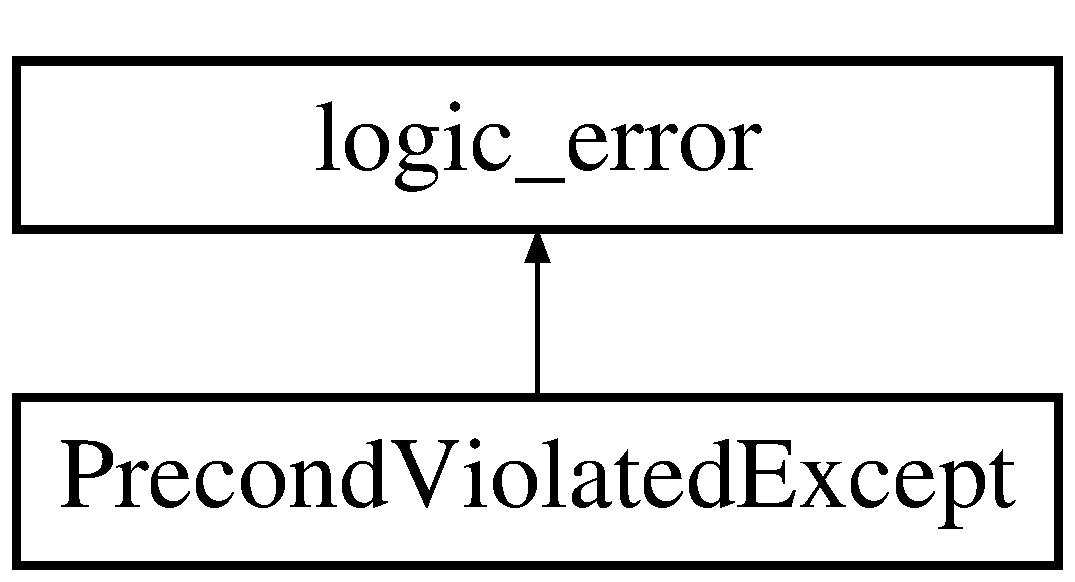
\includegraphics[height=2.000000cm]{class_precond_violated_except}
\end{center}
\end{figure}
\subsubsection*{Public Member Functions}
\begin{DoxyCompactItemize}
\item 
\hypertarget{class_precond_violated_except_a13c9075198f291ffc9a74c0c9b787ecf}{{\bfseries Precond\-Violated\-Except} (const std\-::string \&message=\char`\"{}\char`\"{})}\label{class_precond_violated_except_a13c9075198f291ffc9a74c0c9b787ecf}

\end{DoxyCompactItemize}


The documentation for this class was generated from the following files\-:\begin{DoxyCompactItemize}
\item 
\hyperlink{_precond_violated_except_8h}{Precond\-Violated\-Except.\-h}\item 
\hyperlink{_precond_violated_except_8cpp}{Precond\-Violated\-Except.\-cpp}\end{DoxyCompactItemize}

\section{File Documentation}
\hypertarget{_linked_list_8cpp}{}\subsection{Linked\+List.\+cpp File Reference}
\label{_linked_list_8cpp}\index{Linked\+List.\+cpp@{Linked\+List.\+cpp}}
{\ttfamily \#include \char`\"{}Linked\+List.\+h\char`\"{}}\\*
{\ttfamily \#include \char`\"{}Node.\+h\char`\"{}}\\*
{\ttfamily \#include \char`\"{}Precond\+Violated\+Except.\+h\char`\"{}}\\*


\subsubsection{Detailed Description}
A\+DT list\+: Link-\/based implementation. 
\hypertarget{_linked_list_8h}{\subsection{Linked\-List.\-h File Reference}
\label{_linked_list_8h}\index{Linked\-List.\-h@{Linked\-List.\-h}}
}


Header file for a linked list.  


{\ttfamily \#include \char`\"{}List\-Interface.\-h\char`\"{}}\\*
{\ttfamily \#include \char`\"{}Node.\-h\char`\"{}}\\*
{\ttfamily \#include \char`\"{}Precond\-Violated\-Except.\-h\char`\"{}}\\*
{\ttfamily \#include \char`\"{}Linked\-List.\-cpp\char`\"{}}\\*
\subsubsection*{Classes}
\begin{DoxyCompactItemize}
\item 
class \hyperlink{class_linked_list}{Linked\-List$<$ Item\-Type $>$}
\end{DoxyCompactItemize}


\subsubsection{Detailed Description}
Header file for a linked list. A\-D\-T list\-: Link-\/based implementation. Listing 9-\/2.

establishes functions for list  Created by Frank M. Carrano and Timothy M. Henry. Copyright (c) 2017 Pearson Education, Hoboken, New Jersey. 
\hypertarget{_list_interface_8h}{\subsection{List\-Interface.\-h File Reference}
\label{_list_interface_8h}\index{List\-Interface.\-h@{List\-Interface.\-h}}
}


Interface file for the List A\-D\-T.  


\subsubsection*{Classes}
\begin{DoxyCompactItemize}
\item 
class \hyperlink{class_list_interface}{List\-Interface$<$ Item\-Type $>$}
\end{DoxyCompactItemize}


\subsubsection{Detailed Description}
Interface file for the List A\-D\-T. \begin{DoxyAuthor}{Author}
Rory Pierce
\end{DoxyAuthor}
Specifies the implementation contract of the List A\-D\-T

\begin{DoxyVersion}{Version}
0.\-10
\end{DoxyVersion}
Adapted from Frank M. Carrano and Timothy M. Henry Copyright (c) 2017 Pearson Education, Hoboken, New Jersey. 
\hypertarget{_node_8cpp}{\subsection{Node.\-cpp File Reference}
\label{_node_8cpp}\index{Node.\-cpp@{Node.\-cpp}}
}
{\ttfamily \#include \char`\"{}Node.\-h\char`\"{}}\\*


\subsubsection{Detailed Description}
Listing 4-\/2 
\hypertarget{_node_8h}{\subsection{Node.\-h File Reference}
\label{_node_8h}\index{Node.\-h@{Node.\-h}}
}
{\ttfamily \#include \char`\"{}Node.\-cpp\char`\"{}}\\*
\subsubsection*{Classes}
\begin{DoxyCompactItemize}
\item 
class \hyperlink{class_node}{Node$<$ Item\-Type $>$}
\end{DoxyCompactItemize}


\subsubsection{Detailed Description}
Listing 4-\/1 
\hypertarget{_precond_violated_except_8cpp}{\subsection{Precond\-Violated\-Except.\-cpp File Reference}
\label{_precond_violated_except_8cpp}\index{Precond\-Violated\-Except.\-cpp@{Precond\-Violated\-Except.\-cpp}}
}
{\ttfamily \#include \char`\"{}Precond\-Violated\-Except.\-h\char`\"{}}\\*


\subsubsection{Detailed Description}
Listing 7-\/6. 
\hypertarget{_precond_violated_except_8h}{}\subsection{Precond\+Violated\+Except.\+h File Reference}
\label{_precond_violated_except_8h}\index{Precond\+Violated\+Except.\+h@{Precond\+Violated\+Except.\+h}}
{\ttfamily \#include $<$stdexcept$>$}\\*
{\ttfamily \#include $<$string$>$}\\*
\subsubsection*{Classes}
\begin{DoxyCompactItemize}
\item 
class \hyperlink{class_precond_violated_except}{Precond\+Violated\+Except}
\end{DoxyCompactItemize}


\subsubsection{Detailed Description}
Listing 7-\/5. 
%--- End generated contents ---

% Index
\newpage
\phantomsection
\addcontentsline{toc}{section}{Index}
\printindex

\end{document}
